In diesem Abschnitt wird der Unterschied zwischen einem Framework und einer Bibliothek beleuchtet.

Ein Framework ist eine Softwareplattform, die die Struktur und Architektur des künftigen Softwareprodukts bestimmt.
Jedes Framework enthält ein vorgefertigtes “Gerüst” – die Vorlagen, Standardmodule und APIs, 
die dem Entwickler zur Verfügung stehen.
\footnotemark
\footnotetext{https://it-talents.de/it-wissen/framework/}
Definition der Bibliothek ist:
\begin{quote}
    Bibliothek ist eine Sammlung ähnlicher Objekte, die zur gelegentlichen Verwendung gespeichert werden.\footnotemark
    \footnotetext{https://www.computerweekly.com/de/definition/Bibliothek-Library\#:~:text=In\%20der\%20Informatik\%20bezeichnet\%20der,und\%20physische\%20Speichereinheiten\%20wie\%20Tapes.}
\end{quote}

Der Unterschied zwischen Framework und Bibliothek besteht darin, 
dass bei Framework der geschriebene Code von Framework aufgerufen wird 
und bei Bibliothek der geschriebene Code den Code von Bibliothek  (Inversion Of Control, Kapitel \ref{kap:IoC}).
\footnotemark
\footnotetext{https://martinfowler.com/bliki/InversionOfControl.html}
Beispiele für Bibliotheken sind alle Implementierungen von Netzwerkprotokollen.
Das komplette Verhalten muss vom Clientcode definiert werden.

\begin{figure}[H]
    \centering
    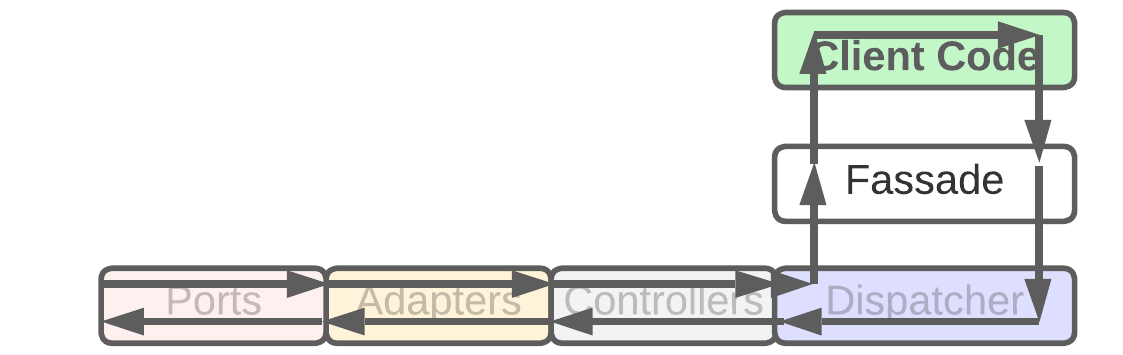
\includegraphics[width=0.9\textwidth]{./images/Dataflow Library.png}
    \caption{Vereinfachte Darstellung des Datenflusses bei einer Bibliothek}
    \label{fig:SimpliedDataflowLibrary}
\end{figure}

In der dargestellten Architektur könnte es zum Beispiel heißen, 
dass das Defaultverhalten (UseCases Schicht) erweitert oder geändert wurde.

\begin{figure}[H]
    \centering
    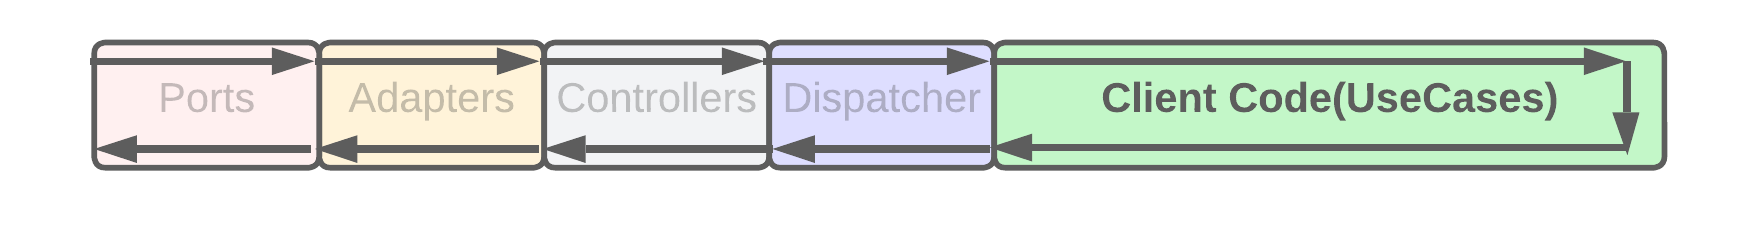
\includegraphics[width=1\textwidth]{./images/Dataflow Framework.png}
    \caption{Vereinfachte Darstellung des Datenflusses bei einem Framework}
    \label{fig:SimpliedDataflowFramework}
\end{figure}

Vergleich des Client Codes von Bibliothek und Framework:

\begin{tabular}{ |l|c|c| } 
    \hline
                                                            & Framework & Bibliothek \\ 
                                                            \hline
    Typen, Konstruktoren                                    & vom Framework vorgegeben  & Selbst geschrieben \\ 
    \hline
    Struktur der Anwendung                                  & vom Framework vorgegeben  & Selbst geschrieben \\
    \hline
    Anteil im Projekt                                       & groß       & gering \\ 
    \hline
\end{tabular}